\documentclass[tp]{lcc}

% add latex preamble
% para la bibliografía se requiere biber y configurar texstudio

% Latex packages
\usepackage[utf8]{inputenc}
\usepackage[T1]{fontenc} % para copiar acentos en español del pdf y permite acentos en las notas
\usepackage[spanish]{babel}
\usepackage[per-mode = symbol]{siunitx} % para manejar las unidades
\usepackage{multimedia} % to add videos with \movie command
\usepackage{multirow}
\usepackage{graphicx}
\usepackage{xcolor}
\usepackage{amsmath} % bmatrix
\usepackage[makeroom]{cancel} % \cancel to cancel terms in math equations
\renewcommand{\CancelColor}{\color{red}} % set red color for \cancel command
\usepackage[caption=false]{subfig} % caption = false elimina la palabra "Figura" del caption
\usepackage{import} % para el comando import (se usa para pdf_tex)
\captionsetup[subfigure]{labelformat=empty} % remover el indice del caption de la subfigura
\usepackage{booktabs} % \toprule \midrule \bottomrule
\usepackage[backend=biber]{biblatex} % set biber to format references. Must configure Biber in Texstudio
\usepackage{csquotes} % to remove warning triggered by biblatex and babel
\usepackage{algorithm} % to put captions to the algorithmics environmets
\usepackage{algpseudocode} % to write algorithm
\usepackage{tikz} % to use tikz
\usetikzlibrary{fit} % to fit a node around other nodes in tikz
\usepackage[export]{adjustbox} % valign in subfloat
\usepackage{colortbl} % to paint cells in a table

% Color commands for annotations
\newcommand\TODO[1]{\textbf{\textcolor{red}{#1}}} %  TODO notes

% Graphic paths
\graphicspath{{./images/}}

% listings configuration for C code
\usepackage{listings} % code
\definecolor{commentgreen}{RGB}{2,112,10}
\definecolor{eminence}{RGB}{108,48,130}
\definecolor{weborange}{RGB}{255,165,0}
\definecolor{frenchplum}{RGB}{129,20,83}

\lstset{ % spanish characters for listings package
	inputencoding=latin1,
    columns=fullflexible,
	breaklines=true,
	tabsize=2,
	showstringspaces=false,
	basicstyle=\ttfamily,
	backgroundcolor=\color{lightgray}, % Choose background color
	literate={á}{{\'a}}1
	{ã}{{\~a}}1
	{é}{{\'e}}1
	{ó}{{\'o}}1
	{í}{{\'i}}1
	{ñ}{{\~n}}1
	{¡}{{!`}}1
	{¿}{{?`}}1
	{ú}{{\'u}}1
	{Í}{{\'I}}1
	{Ó}{{\'O}}1
    {-}{-}1
}

\lstdefinestyle{cpp}{ % spanish characters for listings package
    language=C++,
   	commentstyle=\color{commentgreen},
    keywordstyle=\color{eminence},
    stringstyle=\color{red},
    emph={int,char,double,float,unsigned,void,bool},
    emphstyle={\color{blue}}
}

\lstdefinestyle{bash}{ % spanish characters for listings package
	language=Bash
}

\lstdefinestyle{xml}{
	language=XML,
	morekeywords={encoding,xs:schema,xs:element,xs:complexType,xs:sequence,xs:attribute}
}

\lstdefinestyle{cmake}{
	language=make, % there is no cmake support in listings
}

\lstdefinestyle{python}{
    language=python,
}


%%%%% PARA QUE EN LAS TABLAS SE PUEDA PONER UN SALTO DE LINEA DENTRO DE UNA CELDA
\newcommand{\specialcell}[2][c]{%
    \begin{tiny}
        \begin{tabular}[#1]{@{}c@{}}#2\end{tabular}  
    \end{tiny}
}
%%%%%%%%%%%%%%%%%%%%%%%%%%%%%%%%%%%%%%%%%%%%%%%%%%%%%%%%%%%%%%%%%%%%%%%%

%%%%% PARA QUE LAS TABLAS TENGAN TODAS LAS COLUMNAS CENTRADAS Y DE IGUAL TAMAÑO
\usepackage{tabularx}
\renewcommand{\tabularxcolumn}[1]{>{\centering\arraybackslash}m{#1}}
%%%%%%%%%%%%%%%%%%%%%%%%%%%%%%%%%%%%%%%%%%%%%%%%%%%%%%%%%%%%%%%%%%%%%%%%



% add math preamble
\usepackage{amsmath}
\usepackage{amssymb}
\usepackage{amsopn}
\usepackage{mathtools}

% math
\renewcommand{\vec}[1]{\boldsymbol{\mathbf{#1}}}
\newcommand{\norm}[1]{\lVert#1\rVert}

% Declare arg max and arg min functionss
\DeclareMathOperator*{\argmax}{arg\,max}
\DeclareMathOperator*{\argmin}{arg\,min}

% Homogeneous decoration function
\newcommand{\homo}[1]{\dot{#1}}


% Declare projection as math function
\DeclareMathOperator{\proj}{proj}
\newcommand{\fromCoord}[2]{{#1}_\mathrm{#2}}
\newcommand{\toCoord}[2]{\prescript{\mathrm{#2}}{}{#1}}
\newcommand{\worldCoordSystem}{\mathrm{w}}
\newcommand{\bodyCoordSystem}{\mathrm{B}}
\newcommand{\cameraCoordSystem}{\mathrm{c}}
\newcommand{\point}{\vec{p}}
\newcommand{\worldPoint}{\toCoord{\point}{\worldCoordSystem}}
\newcommand{\imagePoint}{\vec{u}}
\newcommand{\cameraPoint}{\toCoord{\point}{\cameraCoordSystem}}
\newcommand{\homoWorldPoint}{\toCoord{\homo{\point}}{\worldCoordSystem}}
\newcommand{\homoImagePoint}{\homo{\imagePoint}}
\newcommand{\homoCameraPoint}{\toCoord{\homo{\point}}{\cameraCoordSystem}}
\newcommand{\measurement}{\vec{z}}
\newcommand{\prediction}{\hat{\vec{z}}}
\newcommand{\seMatrix}{\vec{\xi}}
\newcommand{\transform}[2]{\toCoord{\fromCoord{\seMatrix}{#2}}{#1}}
\newcommand{\pointCoord}[1]{\toCoord{\point}{#1}}
\newcommand{\rotation}{\vec{R}}
\newcommand{\rotationCoord}[2]{\toCoord{\fromCoord{\rotation}{#2}}{#1}}
\newcommand{\translation}{\vec{t}}
\newcommand{\translationCoord}[2]{\toCoord{\fromCoord{\translation}{#2}}{#1}}
\newcommand{\intrinsicMatrix}{\vec{K}}
\newcommand{\principalPoint}{\vec{c}}
\newcommand{\reprojectionError}{u}
\newcommand{\projectionMatrix}{\vec{P}}
\newcommand{\cameraCenter}{\vec{o}}
\newcommand{\essentialMatrix}{\vec{E}}
\newcommand{\inverse}[1]{{#1}^{-1}}

% Motion model
\newcommand{\position}{\vec{p}}
\newcommand{\orientationQuaternion}{\vec{q}}
\newcommand{\predictedPosition}{\hat{\vec{p}}}
\newcommand{\predictedOrientationQuaternion}{\hat{\vec{q}}}
\newcommand{\linearVelocity}{\vec{v}}
\newcommand{\angularVelocity}{\vec{\omega}}

\DeclareMathOperator{\slerpOp}{slerp}
\newcommand{\slerp}[1]{\slerpOp{\left( #1 \right)}}

% Map structure
\newcommand{\map}{M}
\newcommand{\keyframesSet}{K}
\newcommand{\mapPointsSet}{P}
\newcommand{\observedMapPoints}{O}
\newcommand{\covisibilityKeyframes}{CK}
\newcommand{\localMap}{local\_map}



% Bundle Adjutment
\newcommand{\update}{\vec{\delta}}
\newcommand{\incremental}{\hat{\update}}


% Loop Closure names

% scaled operators and letters to fancy view
\newcommand{\sminus}{\scalebox{0.5}[1.0]{$-$}}
\newcommand{\splus}{\scalebox{0.6}[0.6]{$+$}}
\newcommand{\curr}{c}
\newcommand{\sind}[1]{\scalebox{0.6}[0.6]{$#1$}}
\newcommand{\ind}[1]{\scalebox{0.7}[0.7]{$#1$}}

\newcommand{\keyframe}{\vec{K}}
\newcommand{\bowVector}{\vec{v}}
\newcommand{\lcError}{\vec{\Omega}}
\newcommand{\relativeTransformation}{\seMatrix}
\DeclareMathOperator{\interpolate}{interpolate}

\newcommand{\relativeMotion}{\vec{\delta}}
\newcommand{\groundTruth}[1]{{#1}^{*}}



% definición del operador rot()
\DeclareMathOperator{\rotationOp}{rot}
\newcommand{\getRotation}[1]{\rotationOp{\left( #1 \right)}}

\DeclareMathOperator{\translationOp}{trans}
\newcommand{\getTranslation}[1]{\translationOp{\left( #1 \right)}}









\codigo{R-521}
\materia{Robótica Móvil}
\titulo{ROS2 y Simulador Gazebo}

\soluciones
\commentstrue


\usepackage{biblatex}
%\addbibresource{refs.bib}

\begin{document}
\maketitle


\section{Introducción}

El objetivo de este trabajo práctico es comprender el modelo cinemático y la estimación de pose (posición y orientación) mediante el cálculo de odometría de un robot con ruedas de tracción diferencial que se mueve sobre una superficie plana. Para esta tarea se utilizará ROS2 y el simulador Gazebo.\footnote{Este trabajo práctico está basado en el trabajo práctico del curso Fundamentos de Robótica Móvil del Departamento de Ingeniería Electrónica de la Facultad Regional Córdoba de la Universidad Tecnológica Nacional \url{https://www.profesores.frc.utn.edu.ar/electronica/fundamentosroboticamovil}.}


\section{Entrega}
\begin{itemize}
    \item Se debe proveer un repositorio git que contenga el código desarrollado y un archivo \lstinline{README.md} con las instrucciones de compilación y ejecución. Se recomienda hacer una imagen Docker para facilitar la reproducción de los resuldatos.

    \item Se debe entregar un informe en Lyx o \LaTeX\  explicando el trabajo realizado y analizando los resultados obtenidos.
    
    \item En caso de utilizar el framework \url{https://www.theconstructsim.com}, se deberá proporcionar además el link al proyecto.
\end{itemize}

\section{Evaluación}
\begin{itemize}
    \item Haciendo únicamente los ejercicios obligarorios (no opcionales), el trabajo tiene una nota máxima de 8. Los ejercicios opcionales permiten llegar a la nota máxima de 10.
    \item Entregas Fuera de Término: Si la entrega se realiza durante la primer semana luego del plazo, se decuentan 2 puntos. Si la entrega es más tarde que esto último la nota máxima es de 6.
\end{itemize}

\section{Instrucciones de compilación}
Pasos para trabajar en el simulador Gazebo con el robot TurtleBot3. Mas información en: \url{https://navigation.ros.org/getting_started/}

\begin{enumerate}

\item (Opcional) Si no puede trabajar en su propia computadora (con Ubuntu 22.04) entonces realice los siguientes pasos:

\begin{enumerate}
	\item Iniciar sesión en \url{https://www.theconstructsim.com}.
	\item Crea un proyecto ROSject y seleccionar ROS2 {\bf \<distro\>} como distribución.
\end{enumerate}


\item Instalar los paquetes de ROS2 para la simulación del robot TurtleBot3:

Actualizar la lista de paquetes de linux
\begin{lstlisting}[style=bash] Gente, hoy me tengo que retirar temprano (por eso no fui presencial). Nos vemos!
    sudo apt update
\end{lstlisting}

Instalar los paquetes de Nav2 
\begin{lstlisting}[style=bash] 
	sudo apt install ros-<distro>-navigation2
	sudo apt install ros-<distro>-nav2-bringup
\end{lstlisting}

Instalar los paquetes de Turtlebot 3
\begin{lstlisting}[style=bash] 
	sudo apt install ros-<distro>-turtlebot3*
\end{lstlisting}

	\item Incorporar el script \lstinline[style=bash]{dump_odom.py} provisto por la cátedra
	
\end{enumerate}

\section{Ejecución de la simulación}

\begin{enumerate}

\item Setear las variables de entorno:

\begin{lstlisting}[style=bash] 
export TURTLEBOT3_MODEL=waffle
export GAZEBO_MODEL_PATH=$GAZEBO_MODEL_PATH:/opt/ros/<distro>/share/turtlebot3_gazebo/models
\end{lstlisting}
	\item Ejecutar simulación

\begin{lstlisting}[style=bash] 
ros2 launch nav2_bringup tb3_simulation_launch.py headless:=False
\end{lstlisting}


	\item Una vez corriendo, setear la pose inicial del robot desde RViz. Para esto primero presionar el botón ``2D Pose Estimate'' y luego hacer click es la zona donde se encuentra el robot en el mapa. Esto es para que el sistema de localización del robot tenga una semilla inicial de dónde esta. Luego presionar ``Navigaton2 Goal'' y luego hacer click en algún lugar del mapa para indicarle al robot que debe navegar hasta ahí.

	%\item Crear un launch que permita lanzar la simulación pero sin un mapa y sin el sistema de localización. Se recomienda copiar y modificar los archivos \lstinline{tb3_simulation_launch.py} comentando el código relacionado a la localización (\lstinline{slam}) y al mapa (\lstinline{map}); y \lstinline{world_only.model} comentando el código relacionado al modelo del mundo a utilizar. Entre otros cambios, en el archivo launch deberá modificar el path al world modificado.
	
	\item Utilizar el launch y el modelo world provisto por la cátedra  para lanzar la simulación pero sin un mapa y sin el sistema de localización. El launch provisto es una modificación del  archivo \lstinline[style=bash]{tb3_simulation_launch.py} donde se comentó el código relacionado a la localización (\lstinline[style=bash]{slam}) y al mapa (\lstinline[style=bash]{map}). El modelo world \lstinline[style=bash]{world_only.model} resulta de comentar el código relacionado al modelo del mundo a utilizar.
	

	\item Una vez teniendo el robot corriendo en un mundo sin obstáculos y sin un sistema de localización, enviar comandos de velocidad para mover el robot:

	\begin{enumerate}
	\item En una nueva terminal o pestaña, ejecutar el comando:

\begin{lstlisting}[style=bash] 
ros2 topic pub --rate 1 /cmd_vel geometry_msgs/msg/Twist "{linear: {x: 0.2, y: 0.0, z: 0.0}, angular: {x: 0.0, y: 0.0, z: 0.2}}"
\end{lstlisting}

	\item Detener el robot fijando la velocidad lineal y angular a cero.
	\end{enumerate}

\item Comandar el robot con el teclado (teleoperación), para ello ejecutar:

Puede ejecutarse el mismo comando de teleoperación por teclado
\begin{lstlisting}[style=bash] 
ros2 run teleop_twist_keyboard teleop_twist_keyboard
\end{lstlisting}
(ver la información en pantalla y decrementar las velocidades si el moviemiento del robot
resulta demasiado agresivo)
\end{enumerate}


\section{Ejercicios}

\ejercicio  Determinar de forma analítica el radio del camino circular que realiza el robot al ajustar la velocidad lineal y angular a valores constantes. Realizar el cálculo para dos velocidades cualquieras teniendo en cuenta las velocidades máximas del robot.

\begin{nota}
	Los límites de velocidad y los parámetros cinemáticos (el radio de la rueda R y la distancia entre ruedas b) de los diferentes modelos del robot TurtleBot3 se obtienen de las especificaciones\footnote{\url{https://emanual.robotis.com/docs/en/platform/turtlebot3/features/}}.
\end{nota}

\ejercicio  Calcular la velocidad lineal y angular para que el robot realice un camino circular con radio de \SI{1}{\meter}.

\ejercicio  Calcular las velocidades lineales y angulares de las ruedas (izquierda y derecha) del robot para el camino circular del punto anterior.

\ejercicio Generar un registro (log) de odometría y velocidad del robot, para lo cual hay que ejecutar nuevamente la simulación y utilizar el script \lstinline[style=bash]{dump odom.py}. Este script muestra en pantalla 6 columnas con los siguientes datos: tiempo (timestamp), coordenadas x, y, orientación, velocidad lineal y angular. El registro de datos debe ser realizado con el robot en movimiento utilizando teleoperación por teclado. Para guardar los datos generados por el script hay que redireccionar la salida a un archivo como:

\begin{lstlisting}[style=bash] 
./dump_odom.py > log.txt
\end{lstlisting}

\ejercicio Escribir un script en Python que cargue los datos del archivo log y genere gráficos de:
\begin{enumerate}
	\item el camino seguido por el robot,
	\item la trayectoria (pose respecto al tiempo), y
	\item la velocidad del robot respecto al tiempo.
\end{enumerate} 

\begin{nota}
	Utilizar una relación de aspecto 1:1 para el gráfico del camino y evitar en lo posible el registro de datos iguales a cero.
\end{nota}

\ejercicio (Opcional) Obtener otro registro de datos para un camino circular del robot y graficar el camino y la trayectoria.

\ejercicio (Opcional) Marcar tres puntos cualquiera en el gráfico del camino del robot y sus correspondientes puntos en la trayectoria (Ver Figura~\ref{fig:trajectory_example}). No elegir los puntos de inicio y final del camino.

\begin{figure}[!htbp]
    \centering
    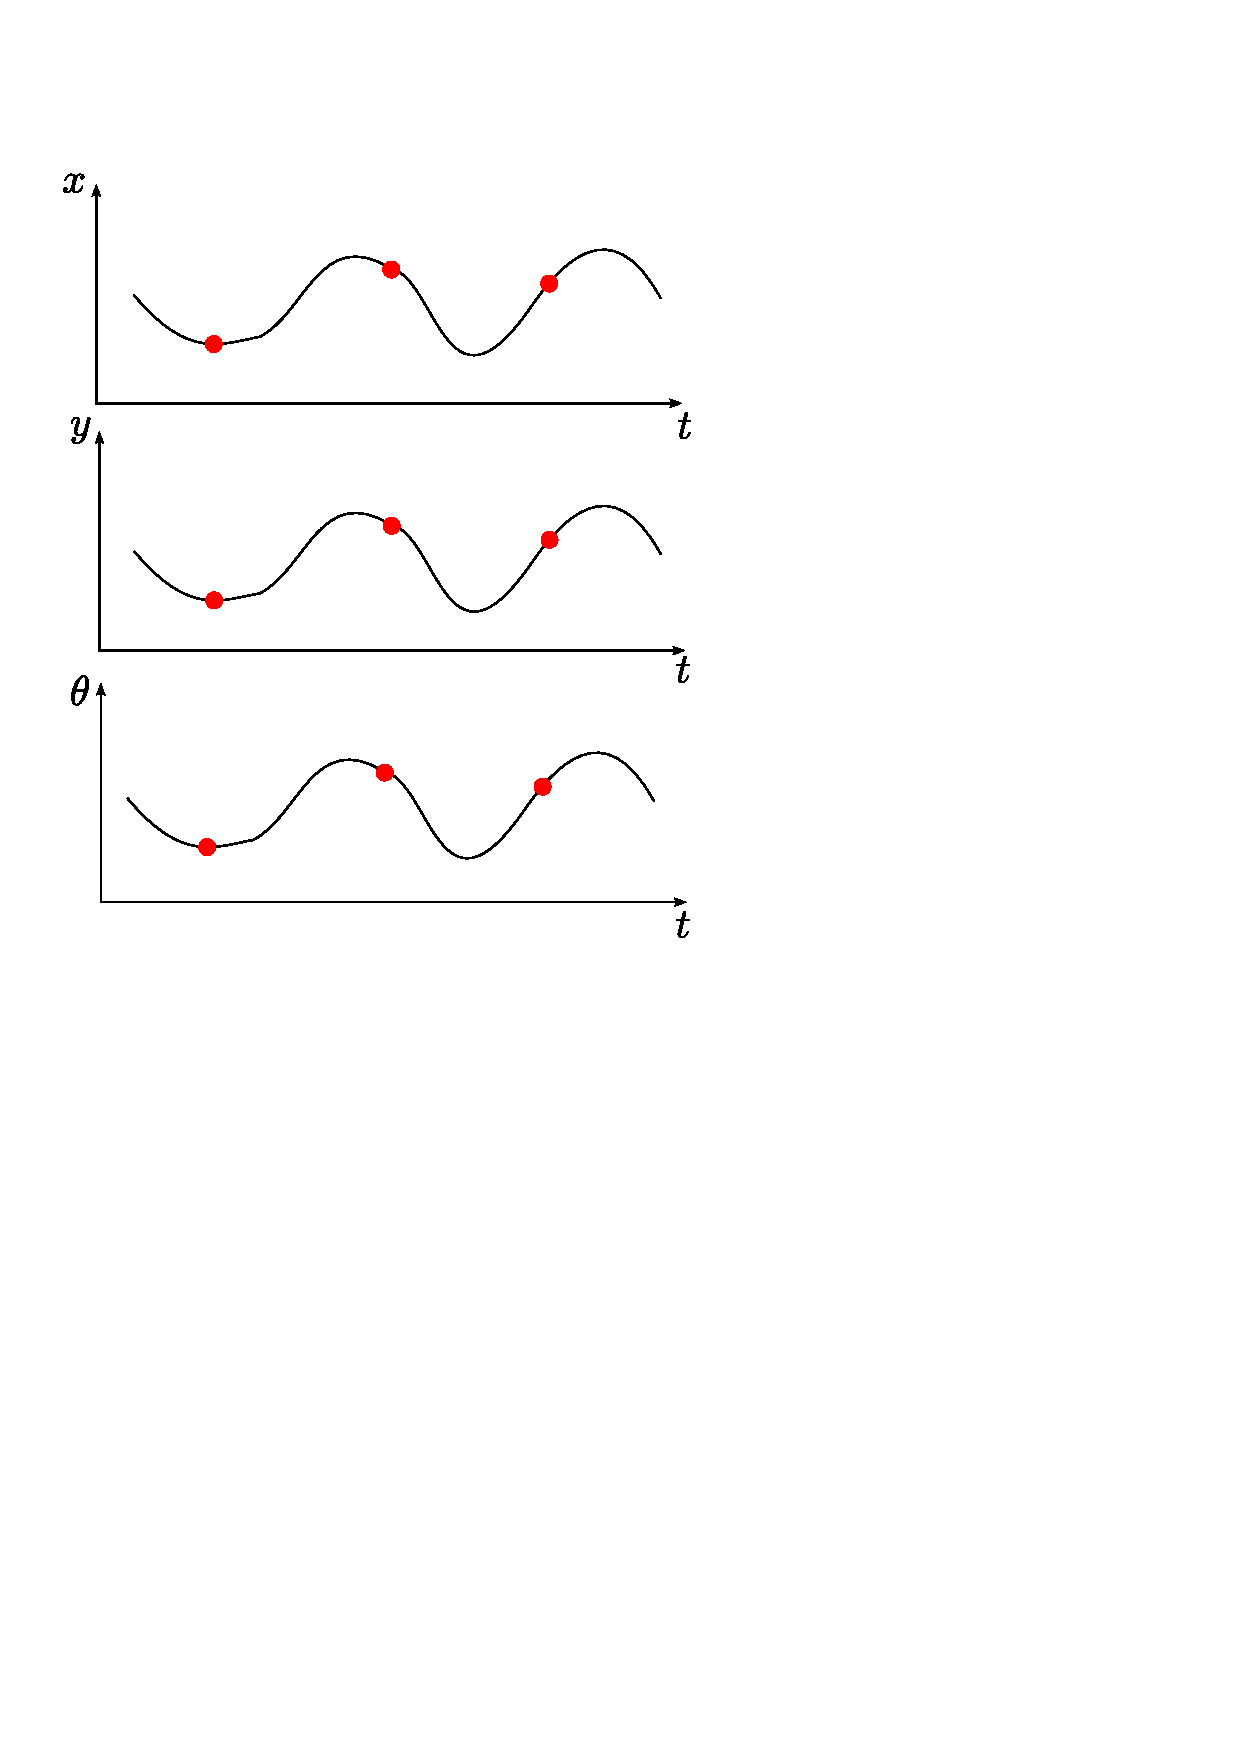
\includegraphics[width=0.7\textwidth]{./images/trajectory_example.pdf}
    \caption{Ejemplo de camino y trayectoria.}
    \label{fig:trajectory_example}
\end{figure}


En base a los gráficos anteriores:

\begin{enumerate}

\item ¿Cuáles son los rangos de valores de las coordenadas x e y y por qué?

\item  ¿Cuál es el rango de valores de la orientación del robot y por qué?

\item Obtener diferentes registros y gráficos para caminos circulares con diferentes valores (positivos y negativos) de velocidades lineales y angulares (utilizar todas las combinaciones de signos posibles). Indicar en los gráficos el sentido de avance del robot.

\item Describir cuál sería la secuencia de comandos de velocidad a aplicar al robot para seguir uno de los caminos mostrados en la Figura~\ref{fig:trajectories} (elegir solo uno).

\begin{nota}
	Para setear los comandos de velocidad por un tiempo determinado se puede utilizar el comando \lstinline[style=bash]{ros2 topic pub} con los argumentos \lstinline[style=bash]{-1} y \lstinline[style=bash]{--keep-alive}.
\end{nota}

\end{enumerate}


\begin{figure}[!htbp]
    \centering
    \subfloat[]
    {
        
\includegraphics[width=0.2\textwidth]{./images/path_a.pdf}
    }
    \hspace{3cm}
    \subfloat[]
    {
        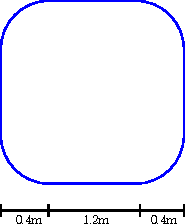
\includegraphics[width=0.2\textwidth]{./images/path_b.pdf}
    }
    \caption{Caminos cuadrados.}
    \label{fig:trajectories}
\end{figure}

\ejercicio Realizar una simulación donde:
\begin{itemize}
    \item El mundo debe contar con varios cilindros de un mismo radio $r$. Los cilindros deben estar distribuidos en el entorno y ser todos observados por el láser del robot al momento de inicio de la simulación.
    \item Utilizar una medición láser para generar un mapa de la escena observada por el robot en simulación. Para esto debe detectar los cilindros en la medición laser obtenida. Cada cilindro es utilizado como un landmark en el mapa virtual del robot. Debe estimar el centro del cilindro, dicha posición será la posición de un landmark en el mapa virtual del robot.
    \item Debe crear un mapa de landmarks, publicarlo y visualizarlo en RVIZ utilizando el marker de cilindro. Obtenga una captura de pantalla de RViz donde se visualice las mediciones del láser y los landmarks reconstruidos.
\end{itemize}





\printbibliography

\end{document}
